\section{2020 年 11 月 21 日答疑记录}

\subsection{二次函数与集合}

\begin{example}
    某渔业公司今年年初用 $98$~万元购进艘渔船用于捕捞, 若该渔船捕捞 $x$ ($x\in \naturalnum^*$) 年后, 包括维修费在内, 所需费用的总和为 $(2x^2 +10x$) 万元, 且该渔船每年的捕捞收入为 $50$ 万元.
    
    (1) 捕捞几年后总利润最大? 最大值是多少? 
    (总利润 $=$ 总收入 $-$ 渔船使用费用总和 $-$ 购船费用)
    
    (2) 捕捞几年后的年平均利润最大? 最大值是多少?
\end{example}
\begin{solution}
    (1) 设 $x$~年后总利润为 $f(x)$~万元, 则
    \[f(x)=50x-(2x^2+10x)-98= -2x^2+40x-98,\quad x\in \naturalnum^*.\]
    因为 $f(x)$ 为二次函数, 且其轴为 $x=10$, 所以最大值为 $f(10)= 102$, 表明捕捞 $10$~年后总利润最大, 最大值是 $102$~万元.
    
    (2) 设 $x$~年后的年平均利润为 $g(x)$~万元, 则
    \[g(x)=\frac{f(x)}x= \frac{-2x^2+40x-98}x
        = 40- 2\biggl(x+\frac{49}x\biggr),\quad x\in \naturalnum^*.\]
    因为 $x+\dfrac{49}x\geqslant 2\sqrt{x\cdot\dfrac{49}x}= 14$, ``$=$'' 成立当且仅当 $x=\dfrac{49}x$ 即 $x=7$, 所以
    \[-2\biggl(x+\frac{49}x\biggr)\leqslant -28,\quad\text{即}\quad
        g(x)= 40- 2\biggl(x+\frac{49}x\biggr)\leqslant 12.\]
    因此捕捞 $7$~年后的年平均利润最大, 最大值是 $12$~万元.
\end{solution}

\begin{example}
    若函数 $f(x)= x^2+ax+b$ 在区间 $[0,1]$ 上的最大值是 $M$, 最小值是 $m$, 则 $M-m$ 的值与 $a$, $b$ 是否有关?
\end{example}
\begin{solution}
    函数 $f(x)$ 是二次函数, 轴为 $x=-\dfrac{a}2$, 即 $a$ 决定了轴的位置. 由二次函数图形容易知道, 当轴恰好过区间 $[0,1]$ 的中点时, $M-m=0$; 否则 $M-n\neq 0$, 且当轴在区间 $[0,1]$ 外离该区间越远时, $M-m$ 越大. 所以 $M-m$ 的值与 $a$ 有关.
    
    当常数 $b$ 变化时, $f(x)$ 的图形相应上下平移, 所以 $M-m$ 固定不变, 即 $M-m$ 的值与 $b$ 无关.
\end{solution}

\begin{example}
    设 $U$ 为全集, $A$, $B$ 是其子集, 则 ``存在集合 $C$ 使得 $A\subseteq C$, $B\subseteq \complement_U C$'' 是 ``$A\cap B=\varnothing$'' 的什么条件?
\end{example}
\begin{solution}
    (此题建议画草图) 因为 $C\cap \complement_U C= \varnothing$, 即 $C$ 与 $\complement_U C$ 是互不相交的集合, 所以由 $A\subseteq C$, $B\subseteq \complement_U C$ 可知 $A$ 与 $B$ 也是互不相交的集合, 即 $A\cap B=\varnothing$.
    
    反之, 若 $A\cap B=\varnothing$, 即 $A$ 与 $B$ 互不相交, 可取 $C=A$ (有多种取法), 此时必有 $A\subseteq C$, $B\subseteq \complement_U C$.
    
    \begin{center}
        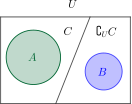
\includegraphics[scale=1]{2020-1206-0940-crop}
    \end{center}
\end{solution}

\subsection{幂、指数与对数}

常用的幂 (指数) 的运算法则有 (以下均假设 $a>0$, $m$, $n\in\realnum$):
\[\begin{gathered}
    a^m\cdot a^n= a^{m+n},\quad \frac{a^m}{a^n}= a^{m-n},\quad 
        (a^m)^n= a^{mn},\quad (ab)^m= a^mb^m,\\
    a^0= 1,\quad a^{-n}= \frac1{a^n},\quad a^{\frac1m}=\sqrt[m]{a}.
    \end{gathered}\]
以上法则中, 前四个可以按 $m$, $n$ 为正整数记忆, 后三个可以由前三个得到. 最后两个可以简记为: 指数中的负号表示 ``取倒数'', 分数表示 ``开方''. 此外, 这些法则还可以嵌套使用, 比如
\[a^{-\frac1m}= \frac1{\sqrt[m]{a}},\quad
    a^{\frac{m}n}= (a^m)^\frac1n= \sqrt[n]{a^m}.\]
    
常用的对数运算法则见 ``2020 年 11 月 8 日答疑记录'' 的第二部分.

\begin{example}
    计算: 
    (1) $2\sqrt{3}\times 3\sqrt[3]{1.5}\times \sqrt[6]{12}$;\qquad
    (2) $32^{-\frac35}- \biggl(2\dfrac{10}{27}\biggr)^{-\frac23}+ 0.5^{-2}$.
\end{example}
\begin{solution}
    根据指数的运算法则,
    \[\begin{aligned}
        2\sqrt{3}\times 3\sqrt[3]{1.5}\times \sqrt[6]{12}
        &= 2\times 3^{\frac12}\times 3\times 
            \biggl(\frac32\biggr)^{\frac13}\times
            (2^2\times 3)^{\frac16}\\
        &= 2^{1-\frac13+\frac26}\times 3^{\frac12+1+\frac13+\frac16}\\
        &= 2\times 3^2= 18,\\
        32^{-\frac35}- \biggl(2\frac{10}{27}\biggr)^{-\frac23}+ 0.5^{-2}
        &= 2^{5\times(-\frac35)}+ \biggl(\frac{64}{27}\biggr)^{-\frac23}+ 2^{(-1)\times(-2)}\\
        &= 2^{-3}+ \frac{3^{3\times\frac23}}{2^{6\times\frac23}}+ 2^2\\
        &= \frac18- \frac9{16}+ 4= \frac{57}{16}.
    \end{aligned}\]
\end{solution}

计算指数式, 一般先化为整数表示, 即小数化最简分数, 根式化分数指数, 同时注意分解质因数, 然后合并同底数的指数即可.

幂函数 $y= x^a$ (均取由 $a$ 对应的自然定义域) 的大致图形如下:

    \begin{center}
        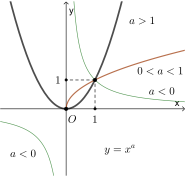
\includegraphics[scale=1]{2020-1206-1110-crop}
    \end{center}

为了整洁起见, 图中并未画出 $a=0$ (对应 $y=1$) 和 $a=1$ (对应 $y=x$) 的情形, 且对 $0<a<1$ 只画了 $x>0$ 对应的图形. 由图可知, 幂函数 $y= x^a$ 的特征有

(1) 当 $a<0$ 且为整数时, 图形有两支, 且以 $x$~轴和 $y$~轴为渐近线, 函数分别在 $(-\infty,0)$ 和 $(0,+\infty)$ 上单调递减; 

(2) 当 $a>0$ 时, 在第一象限内, 函数单调递增, 且 $a$ 越大, 函数值增加速度越快;
 
(3) 恒过点 $(1,1)$ (因为 $1^a=1$).

指数函数 $y= a^x$ ($x\in\realnum$, $a>0$ 且 $a\neq 1$) 的大致图形如下:

    \begin{center}
        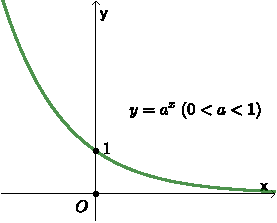
\includegraphics[scale=1]{2020-1206-1030-crop}\qquad
        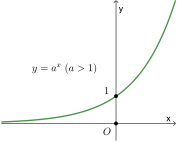
\includegraphics[scale=1]{2020-1206-1040-crop}
    \end{center}

由图可知, 指数函数 $y= a^x$ 的特征有

(1) 当 $0<a<1$ 时, 函数单调递减; 当 $a>1$ 时, 函数单调递增;
 
(2) 恒过点 $(0,1)$ (因为 $a^0=1$), 且以 $x$~轴为渐近线.

指数函数 $y= \log_a x$ ($x$, $a>0$ 且 $a\neq 1$) 的大致图形如下:

    \begin{center}
        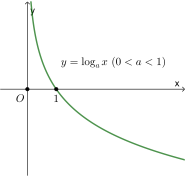
\includegraphics[scale=1]{2020-1206-1050-crop}\qquad
        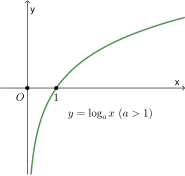
\includegraphics[scale=1]{2020-1206-1100-crop}
    \end{center}

由图可知, 对数函数 $y= \log_a x$ 的特征有

(1) 当 $0<a<1$ 时, 函数单调递减; 当 $a>1$ 时, 函数单调递增;
 
(2) 恒过点 $(1,0)$ (因为 $\log_a 1=0$), 且以 $y$~轴为渐近线.

\begin{remark}
    (1) 指数函数 $y= a^x$ 的定义域为 $\realnum$, 即对 $x$ 没有限制, 而对数函数 $y= \log_a x$ 的自然定义域是 $(0,+\infty)$.
    
    (2) 幂函数 $y= x^a$ 中自变量 $x$ 为底数, 指数函数 $y= a^x$ 中自变量 $x$ 为指数. 
\end{remark}

\begin{example}
    比大小: (1) $a=1$, $b=0.3^2$, $c=2^{0.3}$;
    
    (2) $a= 3^{1.2}$, $b=1.2^0$, $c= \biggl(\dfrac13\biggr)^{-0.9}$;
    
    (3) $a=1.7^{\frac35}$, $b=0.7^{-\frac35}$, $c=0.7^{\frac35}$;
    
    (4) $a=\sqrt[3]{3}$, $b=6^{\frac13}$, $c=2^{-\frac13}$.
\end{example}
\begin{solution}
    (1) 因为 $b=0.09<1$, 由指数函数 $y=2^x$ (或幂函数 $y=x^{0.3}$) 的图形知 $c=2^{0.3}>1$, 所以 $b<a<c$.
    
    (2) 因为 $b=1=3^0$, $c= \biggl(\dfrac13\biggr)^{-0.9}= 3^{0.9}$, 所以由指数函数 $y=3^x$ 的图形知 $b<c<a$.
    
    (3) 因为 $b=0.7^{-\frac35}= \biggl(\dfrac1{0.7}\biggr)^{\frac35}$, 而 $1.7> \dfrac1{0.7}$ (为什么?), 所以由幂函数 $y= x^{\frac35}$ 的图形知, $c<b<a$.
    
    (4) 因为 $a=3^{\frac13}$, $b=6^{\frac13}$, $c=\biggl(\dfrac12\biggr)^{\frac13}$, 由幂函数 $y= x^{\frac13}$ 的图形知, $c<a<b$.
\end{solution}

判断多个数的大小, 一般的方法是:

(1) 先确定这些数与 $0$, $1$ 等数的大小, 将它们分类到 $(-\infty,0)$, $(0,1)$, $(1,+\infty)$ 等区间中;

(2) 对各区间中的幂、指数或对数, 再化为同底数或同指数, 根据相应函数的单调性来判断大小.